\documentclass[conference]{IEEEtran}
\IEEEoverridecommandlockouts
\usepackage{cite}
\usepackage{amsmath,amssymb}
\usepackage{graphicx}
\usepackage{booktabs}
\usepackage{array}
\usepackage{xcolor}
\usepackage[hidelinks]{hyperref}
\graphicspath{{../figures/}}

\begin{document}

\title{External Energy Flexibility: Hourly Clean Supply for Inflexible AI Data Centers Using Existing Grid Loads---A Saudi Arabian Case Study}

\author{\IEEEauthorblockN{[Author Name]\IEEEauthorrefmark{1} and [Advisor Name]\IEEEauthorrefmark{1}}
\IEEEauthorblockA{\IEEEauthorrefmark{1}Department of Electrical and Computer Engineering, Texas A\&M University, College Station, TX, USA\\
Email: [email]}}

\maketitle

\begin{abstract}
Artificial-intelligence (AI) data centers are large, nearly constant loads with little internal flexibility. They can be supplied with renewable energy that matches their consumption over a year, but such annual matching leaves most night-time consumption supplied by fossil generation, while achieving hourly matching with batteries is costly. This paper proposes External Energy Flexibility (EEF): the data center procures photovoltaic (PV) energy equal to its annual consumption, injects all of it into the grid, and, through contracts with the grid, has existing flexible loads elsewhere absorb that PV output; in return, the loads reduce their consumption by the data center's load, so that the data center's supply is displaced rather than stored. We define the actors, an hourly accounting rule and a hierarchical control architecture, formulate linear programs, and compare EEF with direct grid supply, annual matching and PV-plus-battery supply on the data center's reliability, emissions and cost. For a 100-MW data center in Riyadh, annual matching achieves only 40.4\% hourly matching. At an 80\% target, EEF keeps the data center's reliability equal to that of the grid, since a failure of the flexible loads only lowers matching; matches the battery's emissions, a third of those under annual matching; and needs 140~MW of flexible power instead of 1{,}027~MWh of batteries. It is cheaper whenever flexibility costs less than about US\$87 per MWh shifted: at US\$50/MWh it costs US\$17.3 million per year versus US\$30.2 million for the battery.
\end{abstract}

\begin{IEEEkeywords}
AI data centers, demand flexibility, hourly matching, 24/7 carbon-free energy, demand response, energy storage, Saudi Arabia.
\end{IEEEkeywords}

\section{Introduction}
Data centers used about 415~TWh, or 1.5\% of global electricity, in 2024, and their consumption is projected to more than double to about 945~TWh by 2030, with AI the main driver~\cite{r40}. In the United States, data centers used 4.4\% of electricity in 2023 and may reach 6.7--12\% by 2028~\cite{r1}. In Saudi Arabia, data centers used about 2.8~TWh (0.85\% of national electricity) in 2024, which could rise to 10.2--42.2~TWh by 2030~\cite{kapsarcdc}, and the national strategy targets about 1.5~GW of capacity by 2030~\cite{r52}. AI facilities draw power that is high and nearly constant: in a 155{,}410-GPU production trace, only about 6\% of facility power was immediately curtailable~\cite{r26}.

Large consumers usually claim clean supply through \emph{annual matching}: procuring renewable energy equal to annual consumption. Evidence shows that this overstates real mitigation~\cite{r12} and that hourly (24/7) matching is required for system-level emission reductions~\cite{r10,r11}; revisions of carbon-accounting rules toward hourly matching are under consultation~\cite{r50}. Hourly matching, however, has so far relied on procured generation and storage~\cite{r11,r14,r16}, whose cost escalates as the matched share approaches 100\%~\cite{r15}, or on the buyer's own load flexibility~\cite{r9,r10}, which AI data centers largely lack~\cite{r26}. Meanwhile, other grid loads---desalination, district cooling, pumping and industry---can shift consumption~\cite{r19,r20,r23}, but their flexibility is procured by system operators for system services~\cite{r17,r18}, not by a consumer to secure its own clean supply.

This paper proposes \emph{External Energy Flexibility} (EEF) to close this gap. Its contributions are: (i) the EEF concept, with its actors, an hourly accounting rule and a hierarchical control architecture; (ii) linear-programming formulations that quantify the hourly matching achievable with external flexibility and the storage it replaces; and (iii) a case study for Riyadh, Saudi Arabia, that compares four supply configurations on the data center's reliability, emissions and cost, and derives the break-even price of flexibility against battery storage.

\section{Related Work}
\emph{Internal data center flexibility} has been studied extensively: workload shifting with local generation~\cite{r2}, server provisioning with power procurement~\cite{r5}, spatio-temporal workload migration for 24/7 matching~\cite{r9}, and AI workload scheduling with colocated renewables~\cite{r8}; reviews organize these methods~\cite{r3}. All draw flexibility from inside the data center. \emph{Hourly matching} studies optimize portfolios of clean generation and storage under uncertainty~\cite{r14,r16} or with power purchase agreements~\cite{r15}, and assess system impacts~\cite{r10,r11}. \emph{Demand-side flexibility} research quantifies the flexibility of loads such as desalination~\cite{r19,r20}, designs procurement by grid operators~\cite{r18}, and relies on customer baselines for verification~\cite{r17}. In Saudi Arabia, industrial demand-response potential is estimated at 7.1--29.9~GW by 2030, but its role in the single-buyer market is undefined~\cite{r23}. The closest work co-locates a \emph{flexible} data center with one desalination plant and uses waste heat to cut cost~\cite{r22}. No study uses the flexibility of existing external loads to provide hourly clean supply to an \emph{inflexible} data center. Table~\ref{tab:lit} contrasts the closest studies.

\begin{table}[!t]
\centering
\caption{Closest Studies Versus This Work}
\label{tab:lit}
\footnotesize
\setlength{\tabcolsep}{3pt}
\begin{tabular}{@{}p{1.55cm}p{1.45cm}p{3.35cm}p{1.2cm}@{}}
\toprule
Study & Load & Means of hourly matching & Region \\
\midrule
Riepin \cite{r9} & Flexible DCs & Generation, storage, own load shifting & Europe \\
Xu \cite{r10} & Generic buyer & Generation, storage, own demand response & Western U.S. \\
Hwang \cite{r14} & Fixed DC & PV, wind, battery, gas, hourly certificates & Korea \\
Ludkovski \cite{r16} & Fixed loads & Solar and wind PPA portfolio & U.S. \\
Yang \cite{r22} & Flexible DC & Co-located desalination (waste heat), PV, storage & Arid coasts \\
Khanal \cite{r27} & DC tiers & Own shifting and curtailment (planner view) & PJM, Korea \\
\midrule
\textbf{This work} & \textbf{Inflexible AI DC} & \textbf{All PV absorbed by existing external loads under contract} & \textbf{Saudi Arabia} \\
\bottomrule
\end{tabular}
\end{table}

\section{The External Energy Flexibility Concept}
\subsection{Actors and Flows}
Fig.~\ref{fig:arch} shows the arrangement. The data center remains fully grid-supplied, so its reliability equals that of the grid. The data center plays no part in absorbing PV output. A PV plant whose annual output equals the data center's annual consumption injects all its energy into the grid and sells it to the single buyer under a power purchase agreement, and the data center buys all its consumption from the grid. Through contracts with the grid and an aggregator, \emph{all} PV output is absorbed by a portfolio of existing flexible loads, which increase their consumption while PV is generating. In return, the same loads reduce their consumption below their baseline by the data center's consumption, and the grid supply they free is credited to the data center. Each load is energy-neutral within its shifting window: it moves, rather than adds, consumption. Because absorption and reduction coincide in daylight hours, the loads' physical deviation from baseline is their net: an increase equal to PV output minus the data center's consumption around midday, and a decrease equal to the data center's consumption at night. For example, at noon with 350~MW of PV output, the loads absorb 350~MW and reduce 100~MW for a 100-MW data center, a net increase of 250~MW; at 02:00 they reduce 100~MW.

\begin{figure*}[!t]
\centering
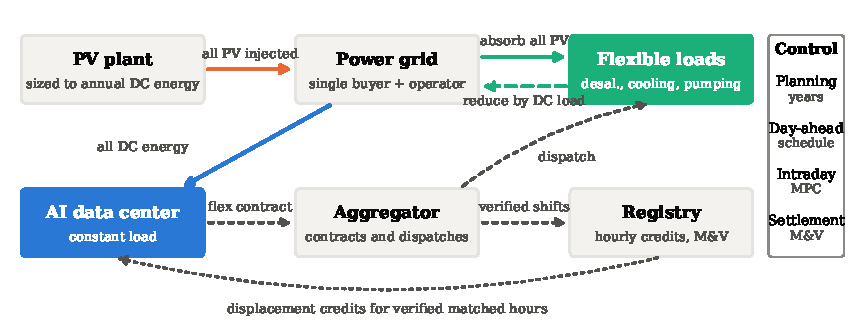
\includegraphics[width=0.92\textwidth]{fig1_architecture.pdf}
\caption{EEF architecture. Solid arrows: energy; dashed: contracts, dispatch and verification; dotted: credits. The control layers act only on the external loads, never on the data center.}
\label{fig:arch}
\end{figure*}

\subsection{Hourly Accounting Rule}
In each hour $t$, the data center is credited with the grid supply freed for it by the flexible loads, up to its consumption, only if (i) the same loads absorbed an equal amount of the PV output within the same window and (ii) their net deviations are verified against their baselines with interval metering. The PV output itself is credited to the flexible loads that absorb it, never to the data center. Credits are recorded in a registry as hourly certificates~\cite{r51}, which prevents double counting with other flexibility services.

\subsection{Control Architecture}
EEF is controlled in four layers. \emph{Planning} (years) sizes the PV plant and the contracted flexible power and energy. \emph{Day-ahead} scheduling forecasts PV output and the data center load, computes the hourly gap and dispatches the cheapest flexibility first, subject to network checks by the system operator. \emph{Intraday} model-predictive correction re-dispatches the loads as forecasts change; any residual error is absorbed by the grid and counted as unmatched. \emph{Settlement} verifies shifts against baselines, issues credits and pays the loads. Because control never acts on the data center, the worst case of EEF is annual matching, with unchanged reliability. This paper addresses the planning layer.

\section{Problem Formulation}
Let $L_t$ be the data center load and $P_t$ the PV output in hour $t \in \mathcal{T}$ ($|\mathcal{T}|=8760$). All PV output is injected into the grid and absorbed by the flexible loads, and all data center consumption is bought from the grid. Netting the loads' absorption of PV and their reduction for the data center in each hour gives a net increase bounded by $s_t=[P_t-L_t]^+$ or a net decrease bounded by $g_t=[L_t-P_t]^+$. The hourly matching (carbon-free energy, CFE) score is
\begin{equation}
\mathrm{CFE}=\frac{\sum_t \min(L_t,P_t)+\sum_t m_t}{\sum_t L_t},
\label{eq:cfe}
\end{equation}
where $m_t \le g_t$ is the shortfall covered by credited flexibility ($m_t=d_t$ for EEF) or by storage discharge ($m_t=b_t$). The first term is the part of the loads' PV absorption that is offset in the same hour by their reduction for the data center; it does not represent consumption of PV by the data center.

\subsection{EEF Model}
The flexible portfolio is represented by one aggregated class with power $P^F$, shiftable energy $D\,P^F$ (duration $D$) and shifting efficiency $\eta$. The net up-shift $u_t$, net down-shift $d_t$ and shifted energy $S_t$ satisfy
\begin{align}
S_t &= (1-\delta_t)\,S_{t-1} + \eta u_t - d_t, \label{eq:state}\\
0 \le u_t &\le \min(P^F, s_t),\quad 0 \le d_t \le \min(P^F, g_t), \label{eq:bounds}\\
0 \le S_t &\le D\,P^F,\qquad S_t = 0\ \ \forall t \in \mathcal{E}, \label{eq:energy}
\end{align}
where $\delta_t=1$ at the start of each 24-h window (06:00) and $\mathcal{E}$ is the set of window-end hours, so each window is energy-neutral. For a target $X$, the minimum contracted flexibility is
\begin{equation}
\min\ P^F \quad \text{s.t. (\ref{eq:state})--(\ref{eq:energy})},\ \ \textstyle\sum_t d_t \ge X\sum_t L_t - \sum_t \min(L_t,P_t).
\label{eq:eefmin}
\end{equation}
For given $P^F$, the maximum CFE is obtained by maximizing $\sum_t d_t$ subject to (\ref{eq:state})--(\ref{eq:energy}).

\subsection{Battery Benchmark (RE+BESS)}
A battery of energy capacity $E$ charges $c_t\le s_t$ from PV output in excess of the data center's same-hour consumption and discharges $b_t\le g_t$:
\begin{equation}
Q_t = Q_{t-1} + \eta_c c_t - b_t/\eta_d,\ \ 0\le Q_t\le E,\ \ Q_0=Q_{|\mathcal{T}|},
\end{equation}
and $\min E$ subject to $\sum_t b_t \ge X\sum_t L_t - \sum_t \min(L_t,P_t)$. Its annual cost is $C^B = c_E E\,(\mathrm{CRF}+\phi)$, with capital cost $c_E$, capital recovery factor CRF and fixed O\&M share $\phi$. Only energy capacity is charged; this favors storage.

\subsection{Break-Even Flexibility Price}
Because both configurations share the same PV plant and grid supply, their cost difference is the cost of hourly matching. EEF is cheaper than storage at target $X$ when the payment per MWh shifted is below
\begin{equation}
\pi^\ast(X) = C^B(X)\,\big/\,\textstyle\sum_t d_t(X).
\end{equation}

\section{Case Study}
Four supply configurations are compared: \emph{GRID}, direct grid supply without clean procurement; \emph{AM}, annual matching, in which a PV plant sized to the data center's annual consumption injects all its output and no flexibility or storage is used; \emph{RE+BESS}, the same PV plant with a battery (Section~IV-B); and \emph{EEF}, the same PV plant with external flexibility (Section~IV-A). In all four, the data center buys its entire consumption from the grid.

A 100-MW AI data center in Riyadh (24.71$^\circ$N, 46.68$^\circ$E) consumes 876~GWh/yr. Hourly PV output for 2020 was obtained from PVGIS-SARAH3 for fixed, optimally tilted crystalline-silicon modules with 14\% losses~\cite{pvgis}; the capacity factor is 20.96\%, so a 477-MWp plant matches the annual consumption. Table~\ref{tab:params} lists the parameters. The models were solved with HiGHS.

\begin{table}[!t]
\centering
\caption{Case-Study Parameters}
\label{tab:params}
\small
\begin{tabular}{@{}lr@{}}
\toprule
Parameter & Value \\
\midrule
Data center load & 100 MW, constant \\
PV plant (annual matching) & 477 MWp; CF 20.96\% \cite{pvgis} \\
Grid tariff (cloud computing) & 0.18 SAR/kWh \cite{kapsarcdc} \\
Battery capital cost, 2030 (4-h) & US\$124/207/338 per kWh \cite{nrelbess2025} \\
Battery round-trip efficiency & 90\% \\
Discount rate, life, fixed O\&M & 8\%, 15 yr, 2.5\%/yr \\
Flexibility shifting efficiency $\eta$ & 0.95 \\
Shifting duration $D$ & 4, 8, 12 h \\
Grid emission factor (average) & 0.568 tCO$_2$/MWh \cite{kfupmghg} \\
\bottomrule
\end{tabular}
\end{table}

\section{Results}
\subsection{Annual Matching Baseline}
Although annual PV energy equals annual consumption, only 40.4\% of the data center's consumption is matched hour by hour. The remaining 521.9~GWh/yr of shortfall equals the net excess of PV output over the data center's consumption around midday (Fig.~\ref{fig:dispatch}).

\subsection{Dispatch Under EEF}
Fig.~\ref{fig:dispatch} shows two days with 150~MW of contracted flexibility and $D=8$~h. The loads' net consumption rises by up to 150~MW around noon and falls by 100~MW at night, raising the annual CFE to 82.0\% with 364.6~GWh/yr shifted.

\begin{figure}[!t]
\centering
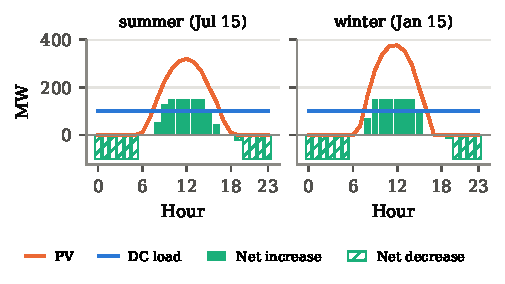
\includegraphics[width=\columnwidth]{fig2_dispatch.pdf}
\caption{Net deviation of the flexible loads from their baseline on a summer and a winter day ($P^F=150$~MW, $D=8$~h). Net decreases are plotted as negative.}
\label{fig:dispatch}
\end{figure}

\subsection{Hourly Matching Versus Contracted Flexibility}
Fig.~\ref{fig:cfe} shows the maximum CFE as a function of contracted flexible power. CFE rises almost linearly to about 80\% at $P^F/L=1.4$ and saturates at 91.2\% above $P^F/L\approx 2.4$; the remaining gap arises on days when PV output is too low to cover the night, since each window must be energy-neutral. With $D\ge 8$~h, the binding constraint is flexible power rather than duration: 8~h and 12~h give identical results, whereas 4~h requires about 1.7 times the power for the same CFE. EEF therefore needs flexible power comparable to the data center load but only moderate shifting duration.

\begin{figure}[!t]
\centering
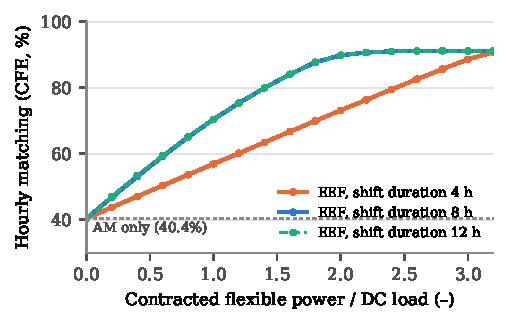
\includegraphics[width=\columnwidth]{fig3_cfe_vs_flex.pdf}
\caption{Hourly matching versus contracted flexible power for three shifting durations.}
\label{fig:cfe}
\end{figure}

\subsection{Three-Pillar Comparison at 80\% Hourly Matching}
Table~\ref{tab:pillars} and Fig.~\ref{fig:pillars} compare the four configurations on the three pillars at an 80\% target; grid energy purchases, US\$42.0~million per year at the cloud-computing tariff, are identical in all of them because the data center always buys its full consumption from the grid.

\emph{Reliability.} The data center is connected to and supplied by the grid at all times in every configuration, so its reliability under EEF is identical to that of direct grid supply: no energy goes unserved, and its availability equals that of the grid. EEF never acts on the data center; if the flexible loads fail to deliver, only hourly matching falls, at worst to the annual-matching level, while the data center's supply is unaffected.

\emph{Sustainability.} EEF and the battery reach the same 80\% matching and the same hourly-accounted emissions, 99.5~kt\,CO$_2$/yr, a third of those under annual matching (296~kt) and a fifth of those under direct grid supply (498~kt). EEF achieves this without building 1{,}027~MWh of new batteries.

\emph{Cost.} The battery costs US\$30.2~million per year (US\$18.1--49.2~million across cost cases), whereas EEF costs US\$17.3~million at US\$50/MWh shifted (US\$8.7--26.0~million at US\$25--75/MWh). EEF is therefore the combination that matches the grid's reliability and the battery's emissions at lower cost, provided that flexibility costs less than the break-even price of about US\$87/MWh shifted.

\emph{Additional grid benefit.} Beyond the three pillars, EEF also relieves the grid: like the battery, it removes most of the load that the data center adds in the evening (16 and 13~MW instead of 100~MW between 19:00 and 23:00), and it removes more after midnight (41 versus 51~MW).

\begin{table}[!t]
\centering
\caption{Three-Pillar Comparison at an 80\% Hourly Matching Target (100-MW Data Center, Riyadh)}
\label{tab:pillars}
\footnotesize
\setlength{\tabcolsep}{3pt}
\begin{tabular}{@{}>{\raggedright\arraybackslash}p{2.6cm}cccc@{}}
\toprule
 & GRID & AM & RE+BESS & EEF \\
\midrule
\multicolumn{5}{@{}l}{\emph{Reliability of the data center}} \\
Supply source & Grid & Grid & Grid & Grid \\
Availability & \multicolumn{4}{c}{identical, equal to that of the grid} \\
Energy not served & 0 & 0 & 0 & 0 \\
If resource fails & -- & -- & CFE falls & CFE $\to$ AM \\
\midrule
\multicolumn{5}{@{}l}{\emph{Sustainability}} \\
CFE (\%) & 0 & 40.4 & 80.0 & 80.0 \\
Emissions (kt CO$_2$/yr) & 498 & 296 & 99.5 & 99.5 \\
New storage (MWh) & 0 & 0 & 1{,}027 & 0 \\
\midrule
\multicolumn{5}{@{}l}{\emph{Cost}} \\
Matching cost (M\$/yr) & 0 & ${\approx}0$ & 30.2 & 17.3$^\ast$ \\
Range (M\$/yr) & -- & -- & 18.1--49.2 & 8.7--26.0$^\ast$ \\
\midrule
\multicolumn{5}{@{}l}{\emph{Additional: impact on the grid}} \\
Load 19--23 h (MW) & 100 & 100 & 13 & 16 \\
Load 00--06 h (MW) & 100 & 100 & 51 & 41 \\
\bottomrule
\multicolumn{5}{@{}p{8.2cm}@{}}{\scriptsize $^\ast$At US\$50 (25--75) per MWh shifted. Load: load added to the grid by the data center and its resources. PV is sold at a price that recovers its cost, so AM adds no net cost. Emissions use the hourly unmatched energy and 0.568~tCO$_2$/MWh~\cite{kfupmghg}.}
\end{tabular}
\end{table}

\begin{figure*}[!t]
\centering
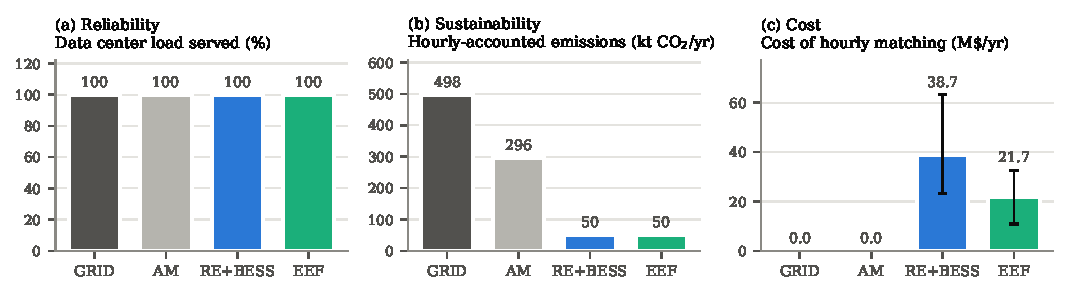
\includegraphics[width=0.95\textwidth]{fig6_pillars.pdf}
\caption{Three-pillar comparison at an 80\% hourly matching target: (a) reliability, as the share of the data center's load served, which is identical in all four configurations because the data center is always supplied by the grid; (b) hourly-accounted emissions; and (c) annual cost of hourly matching (battery: mid case with low--high range; EEF: US\$50/MWh shifted with US\$25--75 range).}
\label{fig:pillars}
\end{figure*}

\subsection{Cost Across Matching Targets}
Reaching 60\%, 80\% and 90\% matching requires 63, 140 and 203~MW of flexibility, or 501, 1{,}027 and 1{,}320~MWh of batteries; at 80\% the battery equals 10.3~h of the data center load. The break-even flexibility price is about US\$86--89/MWh shifted in the mid battery-cost case, rising slightly with the target, and US\$51--146/MWh across the low and high cases; in capacity terms, the mid case corresponds to US\$191--235 per kW-year of contracted flexibility. Fig.~\ref{fig:cost} shows the annual cost of both options across targets. The low-case break-even, about US\$52/MWh, is close to the cloud-computing tariff of US\$48/MWh (18~halalas/kWh) and the industrial tariff of US\$53/MWh~\cite{kapsarcdc}.

\begin{figure}[!t]
\centering
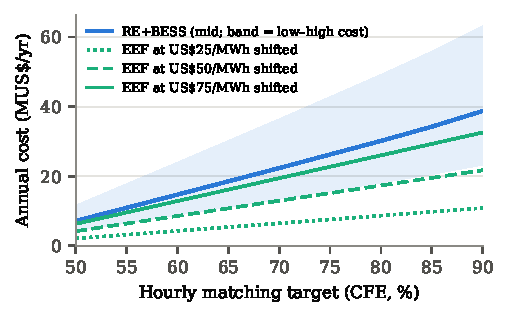
\includegraphics[width=\columnwidth]{fig4_cost.pdf}
\caption{Annual cost of reaching a CFE target with a battery (band: low--high cost) and with EEF at three flexibility prices.}
\label{fig:cost}
\end{figure}

\subsection{Seasonal Performance}
Fig.~\ref{fig:monthly} shows the monthly CFE at an annual target of 80\%. EEF and the battery perform similarly from March to October, and EEF is slightly better in summer (86.6\% versus 85.1\% in June). In winter EEF falls behind (68.6\% versus 71.5\% in December) because external loads shift energy only within a day, whereas the battery can carry energy across days. Annual-matching CFE alone ranges from 34.9\% in December to 44.5\% in June.

\begin{figure}[!t]
\centering
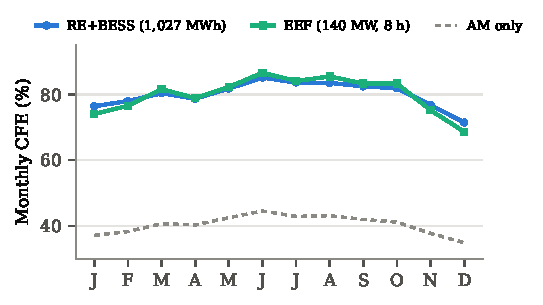
\includegraphics[width=\columnwidth]{fig5_monthly.pdf}
\caption{Monthly hourly matching at an 80\% annual target.}
\label{fig:monthly}
\end{figure}

\subsection{Sensitivity to PV Size and Shifting Efficiency}
Varying the PV plant size and the shifting efficiency $\eta$ shows the following. Oversizing PV by 25--50\% raises the maximum EEF matching from 91.2\% to 93.1--93.7\% and cuts the flexibility needed for 90\% from 203~MW to 162--151~MW, while the battery needed for 90\% falls only from 1{,}320 to 1{,}252--1{,}227~MWh. Lower shifting efficiency increases the flexible power required for 80\% from 140~MW at $\eta=0.95$ to 163~MW at $\eta=0.85$ (132~MW at $\eta=1$) and lowers the maximum matching to 89.3\%, but leaves the energy shifted, and hence the break-even price per MWh shifted, unchanged.


\subsection{Sensitivity to Location}
Repeating the analysis for the NEOM--Oxagon area on the Red Sea coast (27.40$^\circ$N, 35.60$^\circ$E; PV capacity factor 21.37\%) gives nearly identical results: annual matching yields 41.5\% hourly matching; 80\% requires 134~MW of flexibility or a 995-MWh battery; and the mid-case break-even price is US\$86.7/MWh shifted. The maximum CFE reachable with EEF is slightly lower, 89.5\%, so a 90\% target cannot be met by daily shifting alone at this site. The concept and its economics are therefore not specific to one location.

\subsection{National Scale}
At 90\% matching, hourly-accounted emissions fall further to 49.8~kt\,CO$_2$/yr. Scaled to the national target of 1.5~GW of data centers~\cite{r52}, 80\% and 90\% matching would require about 2.1 and 3.0~GW of contracted flexibility, which is within the 7.1--29.9~GW industrial demand-response potential estimated for 2030~\cite{r23}, although that potential is assessed for peak shaving rather than daily shifting.

\section{Discussion and Limitations}
The results show EEF as a combination of the three pillars. On \emph{reliability}, it keeps the data center's supply identical to direct grid supply, and a failure of the flexible loads only lowers matching. On \emph{sustainability}, it delivers the same hourly matching and emissions as a battery and cuts hourly-accounted emissions to a third of those under annual matching, which overstates mitigation~\cite{r12}. On \emph{cost}, it is cheaper than storage whenever flexibility costs less than about US\$87/MWh shifted, a single, transferable figure for negotiating contracts. Its main shortfall is seasonal: within-day shifting cannot carry summer PV into winter nights, so moderate PV oversizing is an effective complement above 90\%, reducing the flexibility needed much more than the storage needed.

The analysis has limitations. Flexibility is represented by one generic class with perfect foresight and one weather year; flexibility costs are unknown and are therefore reported as break-even values; battery costs exclude power-related costs, which favors storage. Emission reductions are reported at the average factor: in Saudi Arabia the marginal generator often changes little with load timing~\cite{r38}, so the benefit of shifting depends on midday PV that would otherwise be curtailed, which becomes more frequent as solar penetration rises~\cite{r23,r44}. Network constraints, baseline accuracy~\cite{r45} and the saturation of flexibility as many data centers compete for it are left to future work.

\section{Conclusion}
External Energy Flexibility lets an inflexible AI data center achieve verifiable hourly clean supply by contracting existing grid loads to absorb all of its PV output and to reduce their consumption by its load, rather than building storage. For a 100-MW data center in Riyadh at 80\% hourly matching, EEF combines the reliability of direct grid supply, the emissions of a battery-backed supply, one third of those under annual matching, and a lower cost than storage whenever flexibility costs less than about US\$87 per MWh shifted. Future work will model a portfolio of heterogeneous flexible loads, the day-ahead and intraday control layers under uncertainty, the contractual framework for single-buyer markets, and the saturation of external flexibility at national scale.

\bibliographystyle{IEEEtran}
\bibliography{../../docs/thesis/refs,refs_extra}

\end{document}
